% =============================================================================
% Volume IV, Lecture 6: Policy Training
% Physical AI: Machine Learning Systems That Sense and Act, Chapter 6
% =============================================================================
% Thesis: every training regime leaves a dependency that the training score
% does not show, so a checkpoint is trusted only inside the region its
% experience supports, and the policy manifest records that region.
% Real running case: OpenAI's Dactyl hand (Andrychowicz et al. 2020), median
% 50 rotations in simulation and 13 on the physical hand (Tables 3 to 5).
% Arithmetic running case: the book's cage-door latch and its three
% checkpoints, latch-bc-01, latch-sim-02 (and latch-res-03), and
% latch-bc-recovery-02 (chapter sections 6.1 to 6.8).
%
% Build:   make deck V=4 D=06_training   (figures: images/make_figs.py)
% Numbers: images/calcs.py prints every derived value with its source.
% Plan:    lecture_map.yml in this folder.
% =============================================================================

\documentclass[aspectratio=169, 12pt]{beamer}
\usepackage{../../assets/beamerthememlsys}
\mlsyssetup{
  volume={Volume IV},
  chapter={Chapter 6},
  chaptertitle={Policy Training},
  layer=brain,
  logo={../../assets/img/logo-mlsysbook.png},
  instlogo={../../assets/img/logo-harvard.png},
}
\usepackage[T1]{fontenc}
\usepackage[scaled=0.9]{helvet}
\usepackage{courier}
\renewcommand{\familydefault}{\sfdefault}
\usepackage{booktabs,amsmath,amssymb}
\usetikzlibrary{arrows.meta,positioning,calc}
\graphicspath{{images/}}
% Generated by calcs.py. Do not edit; edit calcs.py and rerun it.
\defval{dactyl_dof}{24}
\defval{dactyl_sim_trials}{100}
\defval{dactyl_phys_trials}{10}
\defval{dactyl_sim_median}{50}
\defval{dactyl_cap}{50}
\defval{dactyl_all_trials}{50{,} 41{,} 29{,} 27{,} 14{,} 12{,} 6{,} 4{,} 4{,} 1}
\defval{dactyl_all_median}{13}
\defval{dactyl_all_min}{1}
\defval{dactyl_all_max}{50}
\defval{dactyl_gap_words}{four}
\defval{dactyl_none_median}{0}
\defval{dactyl_nophys_median}{2}
\defval{dactyl_noeffects_median}{2}
\defval{dactyl_ff_lstm_median}{3.5}
\defval{dactyl_ff_ff_median}{3}
\defval{dactyl_locked_median}{28.5}
\defval{dactyl_none_hours}{1.5}
\defval{dactyl_all_hours}{50}
\defval{dactyl_none_years}{3}
\defval{dactyl_all_years}{100}
\defval{f_lim}{100}
\defval{f_trip}{15}
\defval{v_guard}{0.03}
\defval{v_fast}{0.10}
\defval{chunk_h}{16}
\defval{step_ms}{25}
\defval{renew_ms}{50}
\defval{act_ms}{40}
\defval{class_f_c}{155}
\defval{act_chunk}{100}
\defval{dp_rollouts}{40}
\defval{ddim_n}{16}
\defval{flow_n}{4}
\defval{enc_ms}{8}
\defval{ddim_ms}{48}
\defval{eval_ms}{2.5}
\defval{flow_ms}{18}
\defval{jitter_ms}{5}
\defval{act_slack_ms}{10}
\defval{ddim_slack_ms}{2}
\defval{ddim_over_ms}{3}
\defval{act_end_ms}{45}
\defval{n_step}{6}
\defval{n_step_ms}{23}
\defval{n_step_room}{6.8}
\defval{budget_ms}{45}
\defval{n_renew}{14}
\defval{n_renew_ms}{43}
\defval{n_renew_room}{14.8}
\defval{decisions}{320}
\defval{rollout_s}{8}
\defval{step_hz}{40}
\defval{gamma}{0.99}
\defval{w_terminal}{0.04}
\defval{horizon_steps}{100}
\defval{horizon_s}{2.5}
\defval{gamma_half}{0.9978}
\defval{w_retained}{0.50}
\defval{step_hz_fast}{80}
\defval{horizon_s_fast}{1.25}
\defval{oxe_used}{970{,}000}
\defval{oxe_used_k}{970}
\defval{plates_words}{three}
\defval{speeds_words}{two}
\defval{cells_words}{six}
\defval{supported}{1}
\defval{supported_words}{one}
\defval{absences}{5}
\defval{trials_e}{6}
\defval{reset_auto_s}{4}
\defval{reset_manual_s}{30}
\defval{exec_days}{92.6}
\defval{auto_days}{138.9}
\defval{manual_days}{439.8}
\defval{manual_days_r}{440}
\defval{reset_pct}{78.9}
\defval{farm_rigs}{14}
\defval{farm_rigs_words}{fourteen}
\defval{farm_days}{31.4}
\defval{reversals_m}{4.0}
\defval{reversals_m_words}{four}
\defval{hil_hours}{2.5}
\defval{trial_s}{12}
\defval{hil_trials}{750}
\defval{hil_factor}{1{,}333}
\defval{hil_reversals}{3{,}000}
\defval{sim_min}{43.4}
\defval{qtopt}{580{,}000}
\defval{farm_attempts}{800{,}000}
\defval{farm_months_words}{two}
\defval{hil_min_h}{1}
\defval{hil_demo_lo}{20}
\defval{hil_demo_hi}{30}
\defval{hil_avg}{20}
\defval{hil_ram_min}{90}
\defval{hil_usb_min}{150}
\defval{robots}{4{,}096}
\defval{steps_upd}{24}
\defval{batch}{98{,}304}
\defval{updates}{1{,}500}
\defval{train_min}{20}
\defval{policy_hz}{50}
\defval{sim_days}{34.1}
\defval{samples_m}{1.47}
\defval{samples_e}{8}
\defval{rate_m}{1.23}
\defval{rate_e}{5}
\defval{mass_kg}{9}
\defval{pen_mm}{2.4}
\defval{k_pen_m}{1.6}
\defval{k_pen_e}{4}
\defval{k_plate_m}{4.0}
\defval{k_plate_e}{5}
\defval{k_star_m}{1.54}
\defval{k_star_e}{5}
\defval{f_sim}{37.5}
\defval{f_rigid}{189.7}
\defval{f_rigid_r}{190}
\defval{f_guard}{56.9}
\defval{plate_x}{25.6}
\defval{rigid_x}{1.9}
\defval{gap_v}{0.20}
\defval{gap_f}{10}
\defval{gap_drive_ms}{8}
\defval{gap_t_sim}{20}
\defval{gap_t_real}{40}
\defval{gap_p99_ms}{49.5}
\defval{gap_travel_mm}{9.9}
\defval{gap_bias_mm}{3.2}
\defval{gap_dropout}{4}
\defval{gap_pixel_pct}{5.5}
\defval{gap_patch_mm}{6}
\defval{gap_tol_mm}{2}
\defval{ft_offset_mm}{1.5}
\defval{ft_steps}{20{,}000}
\defval{ft_active_s}{500}
\defval{ft_pct}{1.5}
\defval{ft_samples}{300}
\defval{t_yield_fast}{2.5}
\defval{t_trip_fast}{0.375}
\defval{t_brake_fast}{2.375}
\defval{t_left_fast}{0.125}

\setcounter{mlsystotalsections}{6}

\title{Policy Training}
\author{Vijay Janapa Reddi}
\institute{Harvard University}
\date{}

% Volume IV diagram roles (rules/volumes/vol4/palette.md)
\definecolor{propblue}{HTML}{2563EB}
\definecolor{nervgreen}{HTML}{059669}
\definecolor{figveto}{HTML}{DC2626}
\definecolor{plantslate}{HTML}{334155}
% A large answer choice for predict and vote slides
\newcommand{\choice}[2]{\textbf{\textcolor{mlsysaccent}{#1}}\enspace #2}
% A goal or takeaway line with its text-free thumbnail
\newcommand{\thumbline}[2]{%
  \begin{minipage}[c]{2.3cm}\centering\safeimg[width=2.2cm,height=0.95cm,keepaspectratio]{#1}\end{minipage}%
  \hspace{0.3cm}\begin{minipage}[c]{0.78\textwidth}#2\end{minipage}}

\begin{document}

% =============================================================================
% TITLE
% =============================================================================
\mlsysnote{[0.5 min] [CORE] Read the thesis aloud once. Lecture 5 built the archive; today trains on it and on three other sources of experience, and asks what each one leaves behind. The notes total about 70 minutes; the frames tagged [OPTIONAL] add about 14, so cutting all of them leaves a complete lecture of about 56 minutes. The planned second lecture splits after \S6.2, at the Interaction divider: learning from demonstrations and logs in the first, learning from interaction and the manifest in the second.}
\mlsystitle{Policy Training}{Every training regime leaves a dependency the training score does not show, so a checkpoint is trusted only inside the region its experience supports.}{cover_training_blueprint.png}

% =============================================================================
% SECTION: TWO POLICIES
% =============================================================================
\mlsysnote{[0.5 min] [CORE] Open on a real robot whose training score and hardware result disagreed by a factor of \val{dactyl_gap_words}.}
\mlsysdivider{Why can a training score rise while the robot gets worse?}{Policy Training, \S6.1 and \S6.4}
\section{Two Policies}

\begin{frame}{A hand trained only in simulation kept breaking on hardware}
  \centering
  \safeimg[width=0.92\textwidth,height=5.1cm,keepaspectratio]{fig06_real_sim2real_dactyl.jpg}\\[0.1cm]
  {\small Dactyl (OpenAI, 2018): a \val{dactyl_dof}-joint Shadow Hand in a camera cage, and its MuJoCo twin.}
  \mlsyscredit{Photo and rendering: OpenAI; Andrychowicz et al., ``Learning Dexterous In-Hand Manipulation,'' IJRR 2020, via Policy Training, \S6.4 (War Story 6.1).}
  \note{[2 min] [CORE] NARRATE: left, the real system: a Shadow Dexterous Hand (\val{dactyl_dof} degrees of freedom, driven through tendons by motors in its forearm) inside an aluminum cage with motion-capture cameras. Right, the MuJoCo simulation (MuJoCo is a physics engine) in which OpenAI trained a reinforcement learning policy to rotate a lettered block to a target face. The policy never practiced on the real hand. Domain randomization, which varies friction, masses, and delays in simulation, is how they hoped it would transfer. The authors reported frequent hardware breakages during physical evaluation, concentrated at the wrist joint under load, and each repair changed tendon tension and friction, so the plant moved under the evaluation. This hand is today's real running case; it returns three times. ENGAGE: what does a simulated hand never do that a real one does? (Expected: wear, break, and change after repair.) WARN: students assume the simulator was crude. It was calibrated against the hand; the gap is in what it omitted. LINK: Lecture 1's causal boundary; a breakage is work that cannot be recalled.}
\end{frame}

\begin{frame}{How many rotations did the real hand manage?}
  \mlsysactivity{Predict}{2 min}
  \centering
  \mlsyssteps[width=0.90\textwidth,height=4.3cm,keepaspectratio]{dactyl_hook_step}{2}\\[0.15cm]
  {\normalsize Same policy, same block, same task. One rotation is one goal face reached.}
  \mlsyscredit{Andrychowicz et al. 2020, Table 3: block (state), all randomizations; \val{dactyl_sim_trials} simulated trials, \val{dactyl_phys_trials} physical trials, sorted values as published. arXiv 1808.00177.}
  \note{[2 min] [CORE] Step 1: the policy's score in its training environment: a median of \val{dactyl_sim_median} consecutive rotations, the cap of the test. ENGAGE: students write a number for the physical hand before the reveal. Most guess 40 to 50, because the policy was trained across thousands of randomized hands. Step 2: the ten physical trials, each dot one trial: \val{dactyl_all_trials}. The median is \val{dactyl_all_median}, and the spread runs from \val{dactyl_all_min} to \val{dactyl_all_max}. The paper's own words: randomizations and calibration narrow the reality gap, but it still exists. WARN: the \val{dactyl_phys_trials} trials were run at different times because of repairs, so they sample several slightly different hands. Today's question is which part of the training experience the score failed to report.}
\end{frame}

\begin{frame}{Recall: what does an archive of successes lack?}
  \mlsysactivity{Retrieval}{1.5 min}
  \centering
  {\Large\bfseries Question of the day}\\[0.3cm]
  {\normalsize Write what a provenance record lists beside its demonstrated cells,\\and why a policy cloned from successes meets states it never saw.}\\[0.4cm]
  \uncover<2->{%
  \begin{mlsyscard}{mlsysaccent}
    \textbf{Known absences} sit beside the supported cells. A robot's own actions choose the states it meets, so a small error carries a cloned policy off the demonstrated states (the second law, endogenous data).
  \end{mlsyscard}}
  \mlsyscredit{Physical Data, \S5.7 and \S5.8; the second law: The Causal Boundary, \S1.10.}
  \note{[1.5 min] [CORE] Retrieval from Lecture 5. Give 60 seconds, then step 2. The provenance record cites the demonstrations and the scenario table, and lists the known absences, the cells with no demonstration. A cloned policy fits actions only at demonstrated states; once its own error moves the arm, it acts from states the archive never held, and Lecture 5 bounded that cost as growing with the square of the horizon. That is the second law, endogenous data: the machine's actions choose its next observations. FLEX: if most students cannot recall ``known absences,'' say it once more, because the declared ODD at the end of today is computed from them.}
\end{frame}

\begin{frame}{Why can a training score rise while the robot gets worse?}
  \small
  By the end of today, you will be able to:\\[0.15cm]
  \thumbline{thumb_dactyl_hook_step2.pdf}{Name the hidden dependency each training regime leaves.}\\[0.15cm]
  \thumbline{thumb_mode_avg_step3.pdf}{Tell mode averaging from drift, and check a decoder's deadline.}\\[0.15cm]
  \thumbline{thumb_reset_wall_step3.pdf}{Price experience on the machine and in a simulator.}\\[0.15cm]
  \thumbline{thumb_odd_step3.pdf}{Compute a declared ODD as supported cells minus omissions.}\\[0.2cm]
  {\footnotesize\textcolor{midgray}{Thread: the second law, endogenous data. Record: the policy manifest.}}
  \note{[1.5 min] [CORE] The title is the driving question and the chapter's own Purpose question. One goal per segment: demonstrations, rewards, interaction (trial and simulation), and the manifest. Name the thread on the bottom line aloud: the second law, endogenous data, which Lecture 5 stated for Part II, a design principle the book raises to a law by choice, unlike the first law, which is physical. Each thumbnail is the picture that teaches its goal. The record chain gains one record today, the policy manifest; Lecture 7's evaluation record takes it as input. FLEX: [CORE].}
\end{frame}

\begin{frame}{Two latch policies open the door, each on a hidden premise}
  \begin{columns}[c]
    \begin{column}{0.30\textwidth}
      \centering
      \safeimg[width=\textwidth,height=4.6cm,keepaspectratio]{tiago-mobile-manipulator.jpg}\\[0.05cm]
      {\scriptsize\textcolor{midgray}{A real mobile manipulator of the running machine's class (PAL TIAGo++).}}
    \end{column}
    \begin{column}{0.67\textwidth}
      \small
      \begin{mlsyscard}{propblue}
        \textbf{latch-bc-01}: cloned from teleoperated openings.\\
        \uncover<2->{\textcolor{figveto}{No recovery data for a sagged door or a displaced plate.}}
      \end{mlsyscard}
      \vspace{0.1cm}
      \begin{mlsyscard}{propblue}
        \textbf{latch-sim-02}: distilled from a simulator teacher trained by reinforcement learning (RL).\\
        \uncover<3->{\textcolor{figveto}{Plunges at \val{v_fast} m/s, because the simulated plate was a soft spring.}}
      \end{mlsyscard}
      \vspace{0.1cm}
      {\footnotesize Both open the door at the nominal plate and the guarded \val{v_guard} m/s approach.}
    \end{column}
  \end{columns}
  \mlsyscredit{Photo: PAL Robotics, CC BY-SA 4.0, Wikimedia Commons (not the book's reference machine). Latch task: Policy Training, \S6.1 (illustrative).}
  \note{[2 min] [CORE] The book's arithmetic case. The running machine is a reference platform, a wheeled base with an arm; the photo shows a real robot of that class. The arm opens a spring-latched cage door against a \val{f_lim} N latch force limit, with a \val{f_trip} N contact tripwire. Both candidates use ACT (Action Chunking with Transformers), which emits \val{chunk_h} setpoints, \val{step_ms} ms apart, per pass. Step 2: latch-bc-01 was cloned from teleoperated openings (behavioral cloning, BC). The archive holds only the nominal plate, so a sagging door puts it in states it never saw. Step 3: latch-sim-02 learned in simulation, where contact was a soft penalty spring, and the reward paid for speed without charging for force. ENGAGE: which candidate would a training score rank higher? (Expected: neither score reveals either premise.) WARN: both are illustrative checkpoints that the chapter constructs; neither is a measured system. LINK: Lecture 5's archive and its known absences.}
\end{frame}

\begin{frame}{Each source of experience leaves its own hidden dependency}
  \centering\small
  \renewcommand{\arraystretch}{1.3}
  \begin{tabular}{@{}p{3.4cm}p{4.2cm}p{5.6cm}@{}}
    \toprule
    \textbf{Experience} & \textbf{What it buys} & \leavevmode\uncover<2->{\textbf{What it silently depends on}} \\
    \midrule
    Demonstrations & expert actions & \leavevmode\uncover<2->{coverage, including recovery} \\
    Logged rewards & better actions from a log & \leavevmode\uncover<2->{actions the log actually tried} \\
    Simulation & cheap, parallel trials & \leavevmode\uncover<2->{the contact solver and what it omits} \\
    Trial on the machine & the real plant & \leavevmode\uncover<2->{days, heat, and drivetrain life} \\
    A pretrained base & broad competence & \leavevmode\uncover<2->{someone else's robots and cells} \\
    \bottomrule
  \end{tabular}\\[0.2cm]
  {\normalsize\uncover<3->{\textcolor{figveto}{\textbf{No loss curve or return reports the right-hand column.}}}}
  \mlsyscredit{Policy Training, \S6.2, table 1, and \S6.10.}
  \note{[2 min] [CORE] Step 1: the five sources of experience the chapter compares, and what each buys. Step 2: the dependency each leaves in the weights. The contact solver is the part of a simulator that computes contact forces. The weights keep what the experience rewarded and forget which experience it was. Step 3: none of the five dependencies appears in a training score. That is the answer to today's question, and each segment opens one row. Demonstrations and pretraining are the Demonstrations and Rewards segments; logged rewards are Rewards; trial and simulation are Interaction. ENGAGE: which row explains Dactyl? (Expected: simulation, the solver and its omissions.) WARN: students read the table as a ranking of regimes. It is not; every row has a cost, and real systems chain several rows.}
\end{frame}

% =============================================================================
% SECTION: DEMONSTRATIONS
% =============================================================================
\mlsysnote{[0.5 min] [CORE] Cloning fails in two separate ways. Separate them first, then price the decoder that fixes one.}
\mlsysdivider{What does a cloned policy do where demonstrators disagree?}{Policy Training, \S6.2.2 to \S6.2.6}
\section{Demonstrations}

\begin{frame}{Squared error sends the policy between two valid routes}
  \begin{columns}[c]
    \begin{column}{0.56\textwidth}
      \centering
      \mlsyssteps[width=\textwidth,height=5.3cm,keepaspectratio]{mode_avg_step}{3}
    \end{column}
    \begin{column}{0.41\textwidth}
      \small
      Half the demos pass left, half pass right.\\[0.3cm]
      \uncover<3->{The squared-error optimum is the mean:\\[0.15cm]
      {\normalsize $\pi^*(o) = \mathbb{E}[a \mid o]$}\\[0.15cm]
      $[v, +\omega]$ and $[v, -\omega]$ average to $[v, 0]$, straight ahead.}
    \end{column}
  \end{columns}
  \mlsyscredit{Policy Training, \S6.2.3, equation 3 and Definition 6.1 (schematic).}
  \note{[2.5 min] [CORE] Step 1: a mobile base, a column ahead. Step 2: demonstrations, every one collision-free: half pass left, half right. Step 3: a deterministic policy trained with mean squared error has one optimal output per observation, the conditional mean of the demonstrated actions ($o$ is the observation, $a$ the action, $v$ forward speed, $\omega$ yaw rate). Left and right yaw cancel to zero, which drives straight into the column, the one path nobody demonstrated. This is mode averaging. More data, more capacity, or longer training move the output closer to the mean. ENGAGE: would a lower validation loss warn you? (Expected: no; the mean minimizes squared error on held-out demonstrations from the same two modes.) WARN: the fix is a different output distribution (a mixture, diffusion, or flow head); a bigger network does not help. In vision the mean is a blurry image; in a robot it is a collision. LINK: Lecture 3 previewed this when it introduced action chunking.}
\end{frame}

\begin{frame}{A diffusion head commits to one route around the block}
  \centering
  \safeimg[width=0.86\textwidth,height=4.1cm,keepaspectratio]{paper_dp_multimodal.png}\\[0.1cm]
  {\small Push-T: from this state the pusher (blue dot) may go left or right of the T. \val{dp_rollouts} rollouts per policy.}
  \mlsyscredit{Chi et al., ``Diffusion Policy,'' RSS 2023 / IJRR 2025, Figure 3 (top-scoring checkpoint of each method), arXiv 2303.04137.}
  \note{[1.5 min] [OPTIONAL] Real rollouts from the Diffusion Policy paper: the task is to push the gray T onto the green target, and from this state either side works. Each panel overlays \val{dp_rollouts} rollouts, colored from dark (start) to bright (end). Diffusion Policy: each rollout commits to one side; both sides appear across rollouts. LSTM-GMM (a recurrent policy with a Gaussian mixture head) and IBC (implicit behavioral cloning) are biased toward one mode. BET (behavior transformer) fails to commit within a rollout, so consecutive actions jump between modes and the trajectories zigzag. ENGAGE: which panel looks like the column slide's straight line? (Expected: none exactly; BET's jitter is what happens when consecutive choices alternate between modes.) WARN: a generated route is still only a candidate; the permission path checks clearance and limits. FLEX: cut if short; the previous slide carries the concept.}
\end{frame}

\begin{frame}{Which failure does a multimodal decoder fix?}
  \mlsysactivity{Vote}{2.5 min}
  \small
  \begin{columns}[T]
    \begin{column}{0.31\textwidth}
      \choice{1}{The base steers straight at the column.}\\[0.25cm]
      \choice{2}{The latch arm drifts until the gripper binds on a sagged door.}\\[0.35cm]
      \uncover<2->{\textbf{Decoder fixes 1.} Only recovery experience fixes 2.}
    \end{column}
    \begin{column}{0.67\textwidth}
      \centering
      \uncover<2->{\safeimg[width=\textwidth,height=5.5cm,keepaspectratio]{drift.pdf}}
    \end{column}
  \end{columns}
  \mlsyscredit{Policy Training, \S6.2.4, figure 1, and Checkpoint 6.1 (schematic).}
  \note{[2.5 min] [CORE] ENGAGE: vote 1, 2, both, or neither. Many vote both. Step 2: mode averaging concerns the action chosen at one observation; drift concerns the states that successive actions reach. A multimodal head picks one route and still drifts. Left panel: the demonstrated tube, where cloning trains; a band just outside where an expert label on a learner-visited state (DAgger, dataset aggregation) still restores the task; and a region beyond where torque limits and the friction cone leave no restoring action, so no label helps. Lecture 5 owns the bound and the recoverability constant; today adds two things. Right panel: the same persistent error integrates once if the policy commands velocity and twice if it commands torque, so torque-level drift grows with the square of time and has no velocity loop beneath it to reject disturbances. WARN: richer decoders are not recovery data. LINK: Lecture 5, compounding error and recoverability.}
\end{frame}

\begin{frame}[fragile]{In LeRobot, ACT predicts \val{act_chunk} setpoints per query}
  \begin{columns}[c]
    \begin{column}{0.52\textwidth}
      \begin{mlsyscode}
\footnotesize\ttfamily
\# configuration\_act.py\\
n\_obs\_steps: int = 1\\
chunk\_size: int = 100\\
n\_action\_steps: int = 100\\
temporal\_ensemble\_coeff = None\\
kl\_weight: float = 10.0\\[0.15cm]
\# modeling\_act.py\\
abs\_err = F.l1\_loss(actions,\\
\hspace*{4.5em}actions\_hat)\\
loss = l1\_loss + mean\_kld * kl\_weight
      \end{mlsyscode}
    \end{column}
    \begin{column}{0.45\textwidth}
      \centering
      \safeimg[width=\textwidth,height=3.5cm,keepaspectratio]{paper_aloha_teleop.png}\\[0.05cm]
      {\footnotesize ALOHA: an operator backdrives leader arms; the follower arms record the demonstration.}
    \end{column}
  \end{columns}
  \mlsyscredit{Code: huggingface/lerobot, src/lerobot/policies/act/, commit df0763a (2026-04-12), Apache-2.0; excerpted. Photo: Zhao et al., RSS 2023, Figure 1, arXiv 2304.13705.}
  \note{[2 min] [OPTIONAL] Real code from the LeRobot implementation of ACT (Zhao et al. 2023), the architecture of both latch policies. One query returns a chunk of \val{act_chunk} future setpoints, and by default all \val{act_chunk} are executed before the next query. The loss compares the whole predicted chunk with the recorded chunk using an L1 (absolute) error, plus a KL term from a conditional variational autoencoder whose latent absorbs differences in operator style. The chapter writes the chunk objective with a Huber penalty, which is quadratic for small errors and linear for large ones, so one tremor or dropout cannot dominate the fit. ENGAGE: does a robust loss make the motion smooth? (Expected: no; it acts on prediction residuals and leaves velocity, acceleration, and jerk unconstrained, so feasibility still needs checks.) WARN: temporal ensembling (averaging overlapping chunks) can average two modes across a seam and bring mode averaging back. Right: the ALOHA rig on which ACT was introduced. LINK: Lecture 3, chunking as a supply lever.}
\end{frame}

\begin{frame}{A \val{ddim_n}-step diffusion head leaves \val{ddim_slack_ms} ms of its \val{renew_ms} ms renewal}
  \centering
  \mlsyssteps[width=0.92\textwidth,height=4.5cm,keepaspectratio]{decoder_step}{3}\\[0.1cm]
  {\small $t_{\text{infer}} = t_{\text{encode}} + N \cdot t_{\text{eval}} = \val{enc_ms} + \val{ddim_n} \times \val{eval_ms} = \val{ddim_ms}$ ms; renewal slack against jitter decides.}
  \mlsyscredit{Policy Training, Napkin Math 6.1 and equation 4 (illustrative heads; ACT \val{act_ms} ms is the machine's p99 target). Values: images/calcs.py.}
  \note{[3 min] [CORE] Worked example, Napkin Math 6.1. Two deadlines: the \val{step_ms} ms setpoint step, for a decoder that must supply every tick itself, and the \val{renew_ms} ms renewal period, for one that runs beside an already admitted chunk prefix. Step 1: ACT decodes the chunk in one pass, \val{act_ms} ms at p99: it misses the \val{step_ms} ms step, so it must run asynchronously, and it leaves \val{act_slack_ms} ms before renewal. Step 2: an illustrative diffusion head sampled with DDIM (denoising diffusion implicit models) in \val{ddim_n} dependent steps: \val{enc_ms} ms to encode the images plus \val{ddim_n} evaluations at \val{eval_ms} ms each, \val{ddim_ms} ms, leaving \val{ddim_slack_ms} ms (derived: (\val{ddim_ms} $-$ \val{enc_ms})/\val{ddim_n} $=$ \val{eval_ms} ms per evaluation). A \val{flow_n}-step flow-matching head at the same cost per evaluation takes \val{flow_ms} ms and fits even the \val{step_ms} ms step. Step 3: add the \val{jitter_ms} ms jitter allowance (jitter is the run-to-run spread of latency). DDIM ends \val{ddim_over_ms} ms past its renewal; ACT ends at \val{act_end_ms} ms, inside. ENGAGE: which number decides schedulability, the mean latency or the slack? (Expected: slack against jitter.) WARN: when a renewal is missed, nothing in the decoder notices. Lecture 4's chunk lease bounds how long the old prefix keeps moving the arm on aging evidence.}
\end{frame}

\begin{frame}{How many denoising steps fit each deadline?}
  \mlsysactivity{Estimate}{2.5 min}
  \centering
  \begin{mlsyscard}{mlsysaccent}
    \normalsize Encoder \val{enc_ms} ms.\enspace Each dependent evaluation \val{eval_ms} ms.\enspace Jitter allowance \val{jitter_ms} ms.
  \end{mlsyscard}
  \vspace{0.2cm}
  {\normalsize What is the largest step count $N$ that fits\ldots}\\[0.3cm]
  \begin{columns}[T]
    \begin{column}{0.45\textwidth}
      \centering
      {\normalsize \textbf{the \val{step_ms} ms setpoint step?}}\\[0.25cm]
      \uncover<2->{{\Large\textbf{\textcolor{mlsysaccent}{\val{n_step}}}}\\[0.05cm]{\small \val{enc_ms} $+$ \val{n_step} $\times$ \val{eval_ms} $=$ \val{n_step_ms} ms}}
    \end{column}
    \begin{column}{0.45\textwidth}
      \centering
      {\normalsize \textbf{the \val{renew_ms} ms renewal, jitter kept free?}}\\[0.25cm]
      \uncover<2->{{\Large\textbf{\textcolor{mlsysaccent}{\val{n_renew}}}}\\[0.05cm]{\small \val{enc_ms} $+$ \val{n_renew} $\times$ \val{eval_ms} $=$ \val{n_renew_ms} ms $\le$ \val{budget_ms} ms}}
    \end{column}
  \end{columns}
  \mlsyscredit{Policy Training, Checkpoint 6.1 (stipulated encoder and per-evaluation cost). Derived: images/calcs.py.}
  \note{[2.5 min] [CORE] ENGAGE: pairs compute both in 90 seconds. Step 2: for the step, $(\val{step_ms} - \val{enc_ms})/\val{eval_ms} = \val{n_step_room}$, so \val{n_step} evaluations (\val{n_step_ms} ms). For the renewal with the jitter allowance kept free, the budget is \val{renew_ms} $-$ \val{jitter_ms} $=$ \val{budget_ms} ms, and $(\val{budget_ms} - \val{enc_ms})/\val{eval_ms} = \val{n_renew_room}$, so \val{n_renew} evaluations (\val{n_renew_ms} ms). Training chooses both the head and its evaluation count, so this arithmetic belongs to training as well as to deployment. WARN: count network evaluations, because a fourth-order Runge-Kutta solver spends four of them per step. Step distillation (training a sampler to reach the same chunk in fewer evaluations) helps only if it keeps the recovery behavior. Land the segment: demonstrations fail by averaging modes and by drifting off the archive; the decoder that fixes averaging must still fit its deadline, and only recovery data fixes drift.}
\end{frame}

% =============================================================================
% SECTION: REWARDS
% =============================================================================
\mlsysnote{[0.5 min] [CORE] When the archive has no answer, a reward can score behavior. The reward then becomes the whole specification.}
\mlsysdivider{What does a reward ask for, and what does a log support?}{Policy Training, \S6.2.1, \S6.2.7, \S6.2.8}
\section{Rewards}

\begin{frame}[fragile]{The reward the engineer writes is the whole objective}
  \centering
  {\large
  $r_t = \underbrace{R_{\text{open}}\,\mathbf{1}[\text{door open}]}_{\text{task}}
  \;\uncover<2->{-\;\underbrace{w_F \max(0, F_t - \val{f_trip}\,\text{N})}_{\text{\textcolor{figveto}{force above tripwire}}}}
  \;-\;\underbrace{c_{\text{step}}}_{\text{time}}$}\\[0.5cm]
  \begin{columns}[T]
    \begin{column}{0.50\textwidth}
      \small
      A Markov decision process (MDP): state, action, physics, and this reward. One opening: \val{decisions} decisions, \val{step_ms} ms apart.\\[0.2cm]
      \uncover<3->{\textbf{latch-sim-02's teacher dropped the force term}, so every millisecond a plunge saved earned reward.}
    \end{column}
    \begin{column}{0.46\textwidth}
      \begin{mlsyscode}
\scriptsize\ttfamily
\# legged\_gym: rewards.scales\\
tracking\_lin\_vel = 1.0\\
lin\_vel\_z = -2.0\\
torques = -0.00001\\
dof\_acc = -2.5e-7\\
collision = -1.\\
action\_rate = -0.01
      \end{mlsyscode}
      {\scriptsize A real reward: one task term, many penalties.}
    \end{column}
  \end{columns}
  \mlsyscredit{Policy Training, \S6.2.1, equation 1 (illustrative). Code: leggedrobotics/legged\_gym, legged\_robot\_config.py, commit 4c345d0 (2021-11-22), BSD-3; excerpted lines.}
  \note{[2 min] [CORE] Step 1: a reward for one opening: a payoff when the door opens, minus a small charge per step for slowness. Step 2: the term that states what to avoid, a penalty per newton above the \val{f_trip} N tripwire. The weights make newtons and seconds commensurable, and choosing them is a design decision the policy manifest records. Step 3: the simulator teacher of latch-sim-02 trained without the force term, so nothing charged for an aggressive approach. Right: real reward weights from legged\_gym, the code behind the ANYmal run later today: one tracking term and a set of penalties on torque, joint acceleration, collisions, and how fast the action changes, each weight a design decision. ENGAGE: on hardware, who measures ``door open''? (Expected: a latch sensor or a learned classifier, and every error in that measurement is a surface the optimizer can exploit.) WARN: adding a shaping term to speed exploration can change what is optimal; only a potential-based term provably leaves the optimal policy unchanged (Ng et al. 1999). For students new to RL: appendix on machine learning, and this chapter owns the RL primer.}
\end{frame}

\begin{frame}{At \val{step_hz} Hz, a discount of \val{gamma} sees only the last \val{horizon_s} s}
  \centering
  \safeimg[width=0.92\textwidth,height=4.6cm,keepaspectratio]{discount.pdf}\\[0.1cm]
  {\small Return $G_t = \sum_j \gamma^j r_{t+j}$ discounts once per decision, so its horizon is counted in steps.}
  \mlsyscredit{Policy Training, \S6.2.1 ($\gamma = \val{gamma}$, \val{step_ms} ms steps, \val{rollout_s} s opening). Derived: images/calcs.py.}
  \note{[1.5 min] [OPTIONAL] The return $G_t$ sums future rewards, each multiplied by the discount $\gamma$ once per step. At $\gamma = \val{gamma}$ the effective horizon $1/(1-\gamma)$ is \val{horizon_steps} steps; at \val{step_ms} ms per step that is \val{horizon_s} s. The door-open reward at the end of an \val{rollout_s} s opening reaches the first decision with weight $\val{gamma}^{\val{decisions}} = \val{w_terminal}$ (red). To keep half its weight across the whole opening, $\gamma$ must be at least \val{gamma_half} (blue; derived as $0.5^{1/\val{decisions}}$). ENGAGE: the team doubles the setpoint rate to \val{step_hz_fast} Hz and keeps $\gamma = \val{gamma}$. What happens to the horizon in seconds? (Expected: it halves to \val{horizon_s_fast} s.) WARN: a discount copied from a 10 Hz benchmark silently changes the task horizon on a faster machine.}
\end{frame}

\begin{frame}{Value and advantage score one action against the usual one}
  \centering
  {\large $Q^\pi(s,a) = r(s,a) + \gamma\,\mathbb{E}\big[Q^\pi(s',a')\big]$}\\[0.3cm]
  {\normalsize $V^\pi(s) = \mathbb{E}_{a\sim\pi}\big[Q^\pi(s,a)\big] \qquad A^\pi(s,a) = Q^\pi(s,a) - V^\pi(s)$}\\[0.45cm]
  \begin{columns}[T]
    \begin{column}{0.44\textwidth}
      \begin{mlsyscard}{propblue}\small
        \textbf{For ML readers:} $Q$ is the return expected after taking $a$; positive $A$ means better than the policy's usual choice.
      \end{mlsyscard}
    \end{column}
    \begin{column}{0.44\textwidth}
      \begin{mlsyscard}{nervgreen}\small
        \textbf{For control readers:} with stage cost $\ell = -r$, $V$ is the negated cost-to-go; LQR solves this recursion in closed form.
      \end{mlsyscard}
    \end{column}
  \end{columns}
  \mlsyscredit{Policy Training, \S6.2.1, equation 2; Bellman 1957; Appendix: Control (LQR and Riccati equations).}
  \note{[1.5 min] [OPTIONAL] The Bellman relation, equation 2. $Q$, the action value, is the reward now plus the discounted value of what follows. $V$, the state value, averages $Q$ over the policy's own actions. The advantage $A$ asks whether an action beats the usual choice from that state. At the plate, a plunge has positive advantage only if its expected return beats the policy's usual approach, and the sign depends on the reward weights. For control students: this is dynamic programming; for linear dynamics and quadratic cost the linear-quadratic regulator solves it in closed form from a Riccati equation. RL keeps the recursion and fits $Q$ and $V$ from sampled transitions because the dynamics are unknown. ENGAGE: which quantity does offline RL fit over a log? (Expected: $Q$, then acts greedily on it, next slide.) FLEX: skip for a class that has seen RL.}
\end{frame}

\begin{frame}{Greedy offline learning trusts actions the log never tried}
  \centering
  \mlsyssteps[width=0.92\textwidth,height=4.5cm,keepaspectratio]{offline_step}{2}\\[0.1cm]
  {\small Offline RL fits a fixed log.\enspace\uncover<2->{A conservative fit lowers values off it but adds no support.}}
  \mlsyscredit{Policy Training, \S6.2.7; Kumar et al., Conservative Q-Learning (CQL), NeurIPS 2020 (schematic).}
  \note{[2 min] [CORE] Offline RL fits $Q$ over a fixed log of transitions with rewards, then picks $\arg\max_a Q(s,a)$, so it can stitch the high-reward pieces of imperfect demonstrations. Step 1: the red fitted curve. Green ticks are actions the log contains. Where the log is empty, the network received no target and can output a spurious high value; the greedy rule finds that peak and proposes an approach nobody tried. The error propagates backward through the Bellman target. Step 2: conservative Q-learning (CQL) adds a penalty that pushes values down everywhere and back up at logged actions, so the pick moves back to the log (blue). The penalty reduces optimism but does not exclude unsupported actions; physical limits stay with the permission path. ENGAGE: the latch log holds nominal successes and labeled tripwire failures. Can CQL produce displaced-plate competence? (Expected: no; those cells are known absences among successes and failures alike.) WARN: CQL's guarantee is a lower bound on expected value under its assumptions; it bounds no single action and certifies no safety property.}
\end{frame}

\begin{frame}{\val{oxe_used_k}K episodes of other robots join none of the latch cells}
  \begin{columns}[c]
    \begin{column}{0.52\textwidth}
      \centering
      \safeimg[width=\textwidth,height=3.4cm,keepaspectratio]{paper_oxe_fig1.png}\\[0.05cm]
      {\footnotesize Lecture 5's Open X-Embodiment archive. OpenVLA-7B trained on \val{oxe_used_k}K of its episodes.}
    \end{column}
    \begin{column}{0.45\textwidth}
      \centering
      \uncover<2->{\safeimg[width=\textwidth,height=4.5cm,keepaspectratio]{cells_support.pdf}\\[0.05cm]
      {\footnotesize \val{supported} supported cell, \val{absences} known absences.}}
    \end{column}
  \end{columns}
  \mlsyscredit{Open X-Embodiment Collaboration, ICRA 2024, Fig. 1, arXiv 2310.08864; Kim et al., OpenVLA, 2024. Cells: Policy Training, \S6.2.8.}
  \note{[2 min] [CORE] Left: Lecture 5's Open X-Embodiment archive, shown by the paper's first figure; recall it in one line and move on. OpenVLA-7B, a vision-language-action model (VLA), trained on \val{oxe_used} of these episodes, and the running machine carries it as its slower intent model (Lecture 3's two-speed brain). Step 2: the latch's scenario table: \val{plates_words} plate positions by \val{speeds_words} approach speeds, \val{cells_words} cells. The campaign supports \val{supported_words}, the nominal plate at the guarded approach. Post-training the generalist on latch demonstrations may make the nominal cell more reliable, and it may propose plausible motions at a displaced plate. None of the pretraining episodes were collected on this arm, door, or gripper, so none joins any cell. Pretraining supplies competence; it supplies no evidence about this machine. ENGAGE: what should the manifest record about the base? (Expected: its weight digest, its pretraining mixture as a known unknown, and the action-space mapping.) WARN: post-training can also erase skills the latch task never exercises (forgetting). LINK: Lecture 5's embodiment contract.}
\end{frame}

\begin{frame}{Which candidate earns the displaced-plate cell?}
  \mlsysactivity{Vote}{2.5 min}
  \normalsize
  \begin{columns}[T]
    \begin{column}{0.62\textwidth}
      \choice{A}{OpenVLA post-trained on the latch demonstrations}\\[0.25cm]
      \choice{B}{Conservative Q-learning over the latch log}\\[0.25cm]
      \choice{C}{latch-bc-01 retrained with reviewed recovery demonstrations at the displaced plate}\\[0.25cm]
      \choice{D}{Simulation RL with friction randomized twice as widely}
    \end{column}
    \begin{column}{0.35\textwidth}
      \uncover<2->{%
      \begin{mlsyscard}{nervgreen}\small
        \textbf{C}, and only as a request. New experience joins the new cell; evaluation must still confirm it.
      \end{mlsyscard}}
    \end{column}
  \end{columns}
  \mlsyscredit{Policy Training, \S6.2.4, \S6.2.7, \S6.2.8, \S6.5, and \S6.8 (latch-bc-recovery-02).}
  \note{[2.5 min] [CORE] ENGAGE: vote, discuss with a neighbor for one minute, vote again. Step 2: C. A is borrowed competence: no pretraining episode joins the cell. B reweights what the log holds; the displaced plate is absent from it. D widens parameters of a model whose contact solver was already wrong; randomization cannot add a mechanism the simulator omits, and its states stay in the omission log. C adds experience on this machine at this cell: the stipulated latch-recovery-02 archive, from which only the stabilized, reviewed segment of each correction becomes a training target (Lecture 5 owns intervention curation; Lecture 14 owns the causal masking rule). WARN: even C only requests the cell. Lecture 7 decides whether the evidence supports it. Land the segment: a reward specifies everything the optimizer will chase, a log supports only the actions it tried, and a pretrained base supports none of this machine's cells.}
\end{frame}

% =============================================================================
% SECTION: INTERACTION
% =============================================================================
\mlsysnote{[0.5 min] [CORE] When no archive has the answer, the robot must generate experience. Price it on the machine, then in simulation.}
\mlsysdivider{What does experience cost on the machine, and in a simulator?}{Policy Training, \S6.3 to \S6.5}
\section{Interaction}

\begin{frame}{A million latch trials take \val{manual_days_r} days with manual resets}
  \centering
  \mlsyssteps[width=0.92\textwidth,height=4.6cm,keepaspectratio]{reset_wall_step}{3}\\[0.1cm]
  {\small Physical RL exploration also costs $\val{reversals_m}\times10^{6}$ load reversals, on any number of rigs.}
  \mlsyscredit{Policy Training, Napkin Math 6.2 (illustrative: $10^{\val{trials_e}}$ trials, \val{rollout_s} s rollout, \val{reset_auto_s} s or \val{reset_manual_s} s reset), \S6.3.1, \S6.4.1. Derived: images/calcs.py.}
  \note{[2 min] [CORE] Worked example, Napkin Math 6.2: campaign time $=$ trials $\times$ (rollout $+$ reset) $/$ rigs. Learning a vision policy from scratch takes on the order of a million trials (QT-Opt, Google's RL grasping system, used over \val{qtopt} real grasps). Step 1: execution alone is \val{exec_days} days of round-the-clock running; automated resets make it \val{auto_days}; manual resets, when a jammed cam needs a technician, make it \val{manual_days}, and the reset is \val{reset_pct} percent of every trial. Step 2: \val{farm_rigs} rigs divide the calendar to \val{farm_days} days, and the wear does not divide. \Val{reversals_m_words} million load reversals still pass through drivetrains, and every trial heats windings toward the \val{class_f_c} degrees C limit of Class F winding insulation (Lecture 2's thermal duty limits). Step 3: two ways out. HIL-SERL's budget of \val{hil_hours} hours at \val{trial_s} s per trial allows \val{hil_trials} trials, \val{hil_factor} times fewer and \val{hil_reversals} reversals. Simulation runs the million openings in \val{sim_min} minutes at a published throughput. ENGAGE: which lever relieves both calendar and wear? (Expected: fewer trials; parallel rigs relieve only the calendar.) WARN: a destabilized trial on hardware delivers its energy before any gradient step can take it back (the first law).}
\end{frame}

\begin{frame}{\Val{farm_rigs_words} arms ran \val{farm_months_words} months for \val{farm_attempts} grasps}
  \begin{columns}[c]
    \begin{column}{0.42\textwidth}
      \centering
      \safeimg[width=\textwidth,height=5.4cm,keepaspectratio]{fig06_real_robot_arm_farm.png}
    \end{column}
    \begin{column}{0.54\textwidth}
      \small
      Each arm had its own gripper, bin, and camera, by day (top) and by night (bottom).\\[0.3cm]
      The farm trained a grasp-success predictor from self-labeled outcomes; it was not RL.\\[0.3cm]
      \textbf{Rigs divide the calendar.} Floor space, power, supervision, and wear grow with every rig.
    \end{column}
  \end{columns}
  \mlsyscredit{Levine et al., ``Learning Hand-Eye Coordination for Robotic Grasping,'' IJRR 2018, via Policy Training, figure 4.}
  \note{[1.5 min] [OPTIONAL] The real thing behind the reset wall. Google's grasping farm: up to \val{farm_rigs} arms ran concurrently, and the cluster collected over \val{farm_attempts} grasp attempts over \val{farm_months_words} months. The farm used self-supervised grasp outcomes to train an offline success predictor, which a servo loop queried; it serves here as a picture of scale. QT-Opt, which did learn grasping by RL, paid the same kind of price for its \val{qtopt} attempts. ENGAGE: what does a technician do in a farm like this? (Expected: clear dropped objects and jams, re-home arms: the manual reset term.) WARN: the bins are the cheap part; gearboxes, bearings, and winding insulation are what the trial count consumes.}
\end{frame}

\begin{frame}{Seeded RL reached full success within \val{hil_hours} hours on the arm}
  \centering
  \safeimg[width=0.86\textwidth,height=4.4cm,keepaspectratio]{paper_hilserl_curves.png}\\[0.05cm]
  {\small Solid: HIL-SERL, RL seeded with \val{hil_demo_lo} to \val{hil_demo_hi} demos. Dashed: HG-DAgger, same human effort.}
  \mlsyscredit{Luo et al., ``Precise and Dexterous Robotic Manipulation via Human-in-the-Loop RL,'' Science Robotics 2025, Figure 5 (top row, running average over \val{hil_avg} episodes), arXiv 2410.21845.}
  \note{[2 min] [OPTIONAL] Published training curves on a real Franka arm. Each line is the success rate, averaged over \val{hil_avg} episodes, against training time. HIL-SERL (human-in-the-loop sample-efficient RL) reaches 100 percent on RAM insertion within about \val{hil_ram_min} minutes and on USB grasp-insert within about \val{hil_usb_min} (read from the figure; the paper reports \val{hil_min_h} to \val{hil_hours} hours per task). Four mechanisms cut the trial count: \val{hil_demo_lo} to \val{hil_demo_hi} teleoperated demonstrations seed the replay buffer; each transition is reused across many updates (off-policy RL with prior data, RLPD); an operator takes over when the policy destabilizes; and a learned binary classifier replaces a hand-written reward. The dashed baseline, HG-DAgger (human-gated DAgger, where corrections become imitation labels) with the same human corrections, does not improve. ENGAGE: what new dependencies did seeding buy? (Expected: support of the demonstrations, the operator's interventions, and the classifier, whose false positives, such as a half-jammed cam read as open, the optimizer will exploit.) WARN: takeovers are authority-record entries; their pre-takeover commands are failure evidence, not imitation targets (Lecture 14).}
\end{frame}

\begin{frame}{\val{robots} simulated ANYmals learned to walk in under \val{train_min} minutes}
  \centering
  \safeimg[width=0.80\textwidth,height=2.65cm,keepaspectratio]{paper_anymal_sim.png}\\[0.05cm]
  \safeimg[width=0.80\textwidth,height=1.9cm,keepaspectratio]{paper_anymal_real.png}\\[0.05cm]
  {\small $\val{robots} \times \val{steps_upd} = \val{batch}$ steps per update; \val{updates} updates; \val{sim_days} simulated days at \val{policy_hz} Hz.}
  \mlsyscredit{Rudin et al., ``Learning to Walk in Minutes Using Massively Parallel Deep RL,'' CoRL 2021, Figures 1 and 7, arXiv 2109.11978. Derived: images/calcs.py.}
  \note{[1.5 min] [OPTIONAL] Top: thousands of simulated ANYmal quadrupeds training at once on one workstation GPU in Isaac Gym, a simulator that keeps every environment in accelerator memory. Bottom: the same policy deployed on the physical robot. The run: \val{robots} robots, \val{steps_upd} steps each per update, \val{batch} transitions per batch, \val{updates} updates of PPO (proximal policy optimization, an on-policy method that needs fresh rollouts in bulk) in under \val{train_min} minutes: $\val{samples_m}\times10^{\val{samples_e}}$ steps, at least $\val{rate_m}\times10^{\val{rate_e}}$ per second, \val{sim_days} days of simulated walking. At that rate the million latch openings take \val{sim_min} minutes. ENGAGE: why might a latch run slower than this? (Expected: contact resolution dominates simulator cost, and a door, cam, and stiff plate are contact-heavy; the authors saw run time vary by a factor of two as robots stopped colliding.) WARN: a throughput figure needs its scene and solver settings; one 2024 simulator benchmark was disputed for disabling self-collisions and using low-accuracy settings.}
\end{frame}

\begin{frame}{What force does a rigid arm put on the latch?}
  \mlsysactivity{Predict}{2.5 min}
  \begin{columns}[c]
    \begin{column}{0.30\textwidth}
      \small
      Fast approach \val{v_fast} m/s, moving mass \val{mass_kg} kg.\\[0.15cm]
      The simulator's spring let the gripper sink \val{pen_mm} mm: \textbf{\val{f_sim} N}.\\[0.2cm]
      \choice{A}{\val{f_sim} N}\\
      \choice{B}{about 60 N}\\
      \choice{C}{about 100 N}\\
      \choice{D}{about \val{f_rigid_r} N}
    \end{column}
    \begin{column}{0.68\textwidth}
      \centering
      \mlsyssteps[width=\textwidth,height=4.7cm,keepaspectratio]{spring_step}{3}\\
      {\small\uncover<3->{$F_{\text{peak}} = v\sqrt{k\,m}$, with arm and plate as springs in series.}}
    \end{column}
  \end{columns}
  \mlsyscredit{Policy Training, Napkin Math 6.3, equations 7 and 8 (illustrative plate stiffness $\val{k_plate_m}\times10^{\val{k_plate_e}}$ N/m, stipulated \val{mass_kg} kg). Derived: images/calcs.py.}
  \note{[2.5 min] [CORE] ENGAGE: vote before step 2; most choose A or B. Step 1: the simulator's penalty spring (contact modeled as a spring that lets surfaces overlap slightly), $\val{k_pen_m}\times10^{\val{k_pen_e}}$ N/m, set by the \val{pen_mm} mm penetration, peaks at \val{f_sim} N, under the \val{f_lim} N limit, so the plunge cost nothing and shortened every episode. Step 2: the real steel plate is \val{plate_x} times stiffer. A rigid arm coasting in at \val{v_fast} m/s peaks at $\val{v_fast}\sqrt{\val{k_plate_m}\times10^{\val{k_plate_e}} \times \val{mass_kg}} = \val{f_rigid}$ N, \val{rigid_x} times the limit: D. Step 3: the real arm is not rigid; its finger pads and joints act as a spring in series with the plate. The curve crosses the limit at an arm stiffness of $\val{k_star_m}\times10^{\val{k_star_e}}$ N/m. Nothing in training measured which side of that line this arm sits on; a push test at the tool decides it. At the guarded \val{v_guard} m/s even a rigid arm peaks at \val{f_guard} N. WARN: the opposite error also happens. A stiff simulated spike that the softer real contact never produces so a policy keyed to the spike keeps pushing. LINK: Lecture 2, transmission compliance.}
\end{frame}

\begin{frame}{The reality gap has four channels, each in its own units}
  \centering
  \mlsyssteps[width=0.97\textwidth,height=5.6cm,keepaspectratio]{gap_vector_step}{4}
  \mlsyscredit{Policy Training, \S6.5, Definition 6.2, figure 7, and table 2 (illustrative linear drive at \val{gap_v} m/s, regulating \val{gap_f} N). Derived: images/calcs.py.}
  \note{[2 min] [CORE] One illustrative scenario, kept apart from the latch: a linear drive approaches a surface at \val{gap_v} m/s and regulates \val{gap_f} N. Step 1, dynamics: an unmodeled \val{gap_drive_ms} ms drive delay and a softer pad halve the force rise, so \val{gap_f} N arrives at \val{gap_t_real} ms instead of \val{gap_t_sim}. Step 2, timing: a p99 actuation delay of \val{gap_p99_ms} ms, against the simulator's zero, carries the mechanism \val{gap_travel_mm} mm before correction begins (\val{gap_v} m/s $\times$ \val{gap_p99_ms} ms, derived), and the lag eats phase margin (Lecture 4). Step 3, sensing: a +\val{gap_bias_mm} mm range bias and a \val{gap_dropout}-frame dropout burst. Step 4, appearance: a \val{gap_pixel_pct} percent pixel difference hides a \val{gap_patch_mm} mm shift of the contact patch, outside a \val{gap_tol_mm} mm tolerance. Each channel fails in its own units, so each needs its own acceptance test. Paired probing measures them: drive the robot and its simulated twin with identical open-loop commands and compare the traces channel by channel. ENGAGE: why not one scalar sim-to-real error? (Expected: it cannot say which channel failed or which interceptor to add.) WARN: a parameter error keeps the equations; an omitted mechanism, such as backlash (play between gear teeth) or bus delay, removes one.}
\end{frame}

\begin{frame}{Dactyl transferred only with randomization and memory}
  \begin{columns}[c]
    \begin{column}{0.60\textwidth}
      \centering
      {\footnotesize\textbf{Randomization held out (Table 4)}}\\
      \safeimg[width=\textwidth,height=5.0cm,keepaspectratio]{dactyl_ablation.pdf}
    \end{column}
    \begin{column}{0.38\textwidth}
      \centering
      \uncover<2->{{\footnotesize\textbf{Network memory (Table 5)}}\\
      \safeimg[width=\textwidth,height=3.4cm,keepaspectratio]{dactyl_memory.pdf}\\[0.1cm]
      {\footnotesize Full randomization took about \val{dactyl_all_hours} h of training; none took \val{dactyl_none_hours} h.}}
    \end{column}
  \end{columns}
  \mlsyscredit{Andrychowicz et al. 2020, Tables 4 and 5 (\val{dactyl_phys_trials} physical trials each, sorted values as published) and \S6.3, arXiv 1808.00177.}
  \note{[2 min] [CORE] Real data from the hook's paper. Left: policies trained with groups of randomizations held out, each tested \val{dactyl_phys_trials} times on the physical hand. All randomizations: median \val{dactyl_all_median}. No randomizations: median \val{dactyl_none_median}. No physics randomization, or no modeled unmodeled effects such as backlash and action delay: median \val{dactyl_nophys_median}. The easiest simulator trained fastest, \val{dactyl_none_hours} hours against about \val{dactyl_all_hours} (\val{dactyl_none_years} against \val{dactyl_all_years} simulated years), and transferred worst; the training ranking inverted on hardware. Step 2: the same randomized training with a feed-forward policy instead of an LSTM (a recurrent network with memory): median \val{dactyl_ff_ff_median} to \val{dactyl_ff_lstm_median} against \val{dactyl_all_median}. Memory lets the policy infer which plant it is on from the recent response, an implicit system identification. ENGAGE: why can randomization not fix a missing mechanism? (Expected: it varies coefficients in the equations the simulator has; it cannot add an equation.) WARN: a range widened by a training curriculum (automatic domain randomization) reflects what the optimizer can master, not the hardware, and never enlarges the declared ODD.}
\end{frame}

\begin{frame}{The student cannot recover a state its sensors never see}
  \centering
  \begin{tikzpicture}[font=\small, box/.style={draw, rounded corners=3pt, minimum height=0.8cm, align=center, line width=0.9pt}]
    \node[box, draw=plantslate, fill=gray!8, text width=3.0cm] (priv) at (0,1.4) {privileged state:\\friction, plate offset,\\contact wrench};
    \node[box, draw=propblue, fill=blue!5, text width=2.2cm] (teach) at (3.6,1.4) {teacher\\(RL, sim)};
    \node[box, draw=plantslate, fill=gray!8, text width=3.0cm] (hist) at (0,-0.6) {onboard sensor\\history};
    \node[box, draw=propblue, fill=blue!5, text width=2.2cm] (stud) at (3.6,-0.6) {student\\(imitates)};
    \draw[-{Stealth}, line width=1pt] (priv) -- (teach);
    \draw[-{Stealth}, line width=1pt] (hist) -- (stud);
    \draw[-{Stealth}, line width=1pt, propblue] (teach) -- node[right, font=\footnotesize]{labels} (stud);
    \draw[dashed, plantslate, line width=1pt] (5.5,2.4) -- (5.5,-1.6);
    \node[font=\footnotesize\bfseries, text=plantslate] at (2.4,2.85) {training in simulation};
    \node[font=\footnotesize\bfseries, text=plantslate] at (8.6,2.85) {on the machine};
    \node[box, draw=propblue, fill=blue!5, text width=2.6cm, dashed] (frozen) at (7.4,-0.6) {frozen student:\\proposal every \val{renew_ms} ms};
    \draw[dashed, figveto, line width=1.2pt] (9.2,0.5) -- (9.2,-1.6) node[below, font=\scriptsize, text=figveto] {proposal boundary};
    \node[box, draw=nervgreen, fill=green!5, text width=1.7cm] (perm) at (10.6,-0.6) {permission\\path};
    \draw[-{Stealth}, line width=1pt, propblue] (frozen) -- (perm);
    \draw[-{Stealth}, line width=1pt] (stud) -- (frozen);
    \node<2->[font=\small, text=figveto, align=center] at (8.6,1.3) {plate offset: unobservable\\from joint history};
  \end{tikzpicture}
  \mlsyscredit{Policy Training, \S6.5.1 and figure 8 (redrawn); Pinto et al. 2018; Lee et al. 2020; Kumar et al. 2021.}
  \note{[1.5 min] [OPTIONAL] The simulator knows things the robot never will: exact friction, the plate's offset, the contact wrench. Teacher-student distillation trains a privileged teacher with RL, then trains a student to imitate it from the onboard sensor history only; asymmetric actor-critic instead gives privileged state only to the critic, which is discarded after training. Only the frozen student crosses to the machine, where its proposals still cross the proposal boundary (Lecture 1) to the permission path. Step 2: a history of commanded effort against measured motion can reveal stiffness or friction from the response. An unobserved geometric offset leaves no distinct signature, so the student cannot learn it just because the teacher knew it. ENGAGE: which privileged quantity can the student recover? (Expected: contact stiffness and friction, from the transient response; the offset stays hidden.) WARN: an auxiliary loss that predicts privileged parameters regularizes the encoder but cannot create information absent from the sensors. Land the segment: trial on the machine costs days and wear; simulation costs fidelity, measured channel by channel; neither is free evidence.}
\end{frame}

% =============================================================================
% SECTION: THE MANIFEST
% =============================================================================
\mlsysnote{[0.5 min] [CORE] Training changes weights. Write down what changed, what supports it, and where it may act.}
\mlsysdivider{Where may a trained checkpoint be trusted?}{Policy Training, \S6.6 to \S6.8}
\section{The Manifest}

\begin{frame}{Does a fine-tuned checkpoint keep its evidence?}
  \mlsysactivity{Diagnose}{2 min}
  \centering
  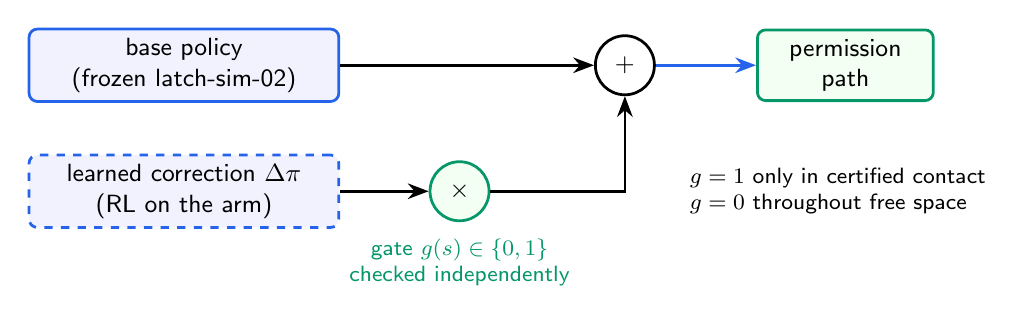
\begin{tikzpicture}[font=\small, box/.style={draw, rounded corners=3pt, minimum height=0.85cm, align=center, line width=1pt}]
    \node[box, draw=propblue, fill=blue!5, text width=3.7cm] (base) at (0,1.0) {base policy\\(frozen latch-sim-02)};
    \node[box, draw=propblue, fill=blue!5, text width=3.7cm, dashed] (res) at (0,-0.6) {learned correction $\Delta\pi$\\(RL on the arm)};
    \node[draw, circle, line width=1pt, draw=nervgreen, fill=green!5, minimum size=0.75cm] (gate) at (3.5,-0.6) {$\times$};
    \node[font=\footnotesize, text=nervgreen, align=center] at (3.5,-1.5) {gate $g(s) \in \{0,1\}$\\checked independently};
    \node[draw, circle, line width=1pt, minimum size=0.75cm] (sum) at (5.6,1.0) {$+$};
    \node[box, draw=nervgreen, fill=green!5, text width=2.0cm] (perm) at (8.4,1.0) {permission\\path};
    \draw[-{Stealth}, line width=1pt] (base) -- (sum);
    \draw[-{Stealth}, line width=1pt] (res) -- (gate);
    \draw[-{Stealth}, line width=1pt] (gate) -| (sum);
    \draw[-{Stealth}, line width=1pt, propblue] (sum) -- (perm);
    \node<2->[font=\footnotesize, align=left, anchor=west] at (6.3,-0.6) {$g = 1$ only in certified contact\\$g = 0$ throughout free space};
  \end{tikzpicture}\\[0.25cm]
  {\small\uncover<3->{\val{ft_steps} steps on the arm: \val{ft_active_s} s of contact; \val{ft_samples} samples above \val{f_trip} N may be a few long contacts.}}\\[0.05cm]
  {\normalsize\uncover<3->{\textbf{No. Changed weights are a new checkpoint; a gate confines where they act.}}}
  \mlsyscredit{Policy Training, \S6.6 and \S6.6.1, equation 11 (latch-res-03, illustrative). Derived: images/calcs.py.}
  \note{[2 min] [CORE] ENGAGE first: do latch-sim-02's trials still count for the fine-tuned weights? Pairs answer in 30 seconds; most say yes for free-space motion. The physical plate sits \val{ft_offset_mm} mm from its simulated position, so the team fine-tunes on the arm. Step 1: latch-res-03 freezes latch-sim-02 and learns an additive correction, multiplied by a binary gate that a separate check evaluates. Step 2: the gate is one only in certified contact and zero in free space, so the correction cannot drift the approach, where training gave it no gradient. Step 3: the run: \val{ft_steps} steps at \val{step_ms} ms, \val{ft_active_s} s of contact. If \val{ft_pct} percent of steps exceed the \val{f_trip} N tripwire, that is \val{ft_samples} samples, but consecutive samples belong to one sustained contact, so count contact events from the force trace. Any update produces a new checkpoint; trials of the old weights say nothing about the new ones. A full-weight update instead needs regression over every operating mode. WARN: a magnitude clip is one limit among several: slew, joint limits, and the stability of the combined loop also need checks. LINK: Lecture 16 applies this rule to release updates.}
\end{frame}

\begin{frame}{The policy manifest records how a checkpoint was produced}
  \begin{columns}[T]
    \begin{column}{0.54\textwidth}
      \footnotesize
      \renewcommand{\arraystretch}{1.1}
      \begin{tabular}{@{}p{2.55cm}p{4.1cm}@{}}
        \toprule
        \textbf{Field} & \textbf{Latch entry} \\
        \midrule
        regime\_sequence & bc-01 $\rightarrow$ sim-02 $\rightarrow$ res-03 \\
        base\_checkpoint & none; digest if any \\
        inference contract & ACT, \val{chunk_h} setpoints, \val{act_ms} ms p99 \\
        data\_support & \val{supported} cell; \val{absences} known absences \\
        omission\_log & soft plate; no bus lag \\
        wear log & rig, contacts, current \\
        \textbf{declared ODD} & \textbf{support minus omissions} \\
        \bottomrule
      \end{tabular}
    \end{column}
    \begin{column}{0.43\textwidth}
      \uncover<2->{%
      {\footnotesize\textbf{A real model card, for comparison}}\\[0.05cm]
      \begin{mlsyscode}
\scriptsize ``trained on \val{oxe_used_k}K robot manipulation episodes from the Open X-Embodiment dataset''\\[0.1cm]
``Out-of-Scope: OpenVLA models do not zero-shot generalize to new (unseen) robot embodiments''
      \end{mlsyscode}
      {\footnotesize The card names its data and its limit. A manifest computes the limit for this machine.}}
    \end{column}
  \end{columns}
  \mlsyscredit{Policy Training, \S6.8 and table 4. Card: huggingface.co/openvla/openvla-7b, README (MIT), retrieved 2026-10-19; excerpted.}
  \note{[2 min] [CORE] Step 1: the fields of the policy manifest, filled for the latch lineage. regime\_sequence lists the stages with checkpoint hashes, losses, and reward weights. base\_checkpoint holds a pretrained base by weight digest, its pretraining mixture as a known unknown. The inference contract holds the head, horizon, evaluation count, and deadline (the decoder slide). data\_support cites Lecture 5's provenance records by digest. The omission log lists what the simulator leaves out and what no paired probe has closed: here the soft plate and the missing actuator bus lag. The adaptation wear log ties fine-tuning to a rig, its contact events, and its motor currents. Step 2: a real model card, OpenVLA's. It names its training data and states a scope limit in words. The manifest goes further: it computes, for this machine, which cells the checkpoint may be evaluated in. ENGAGE: which field would have warned about Dactyl? (Expected: the omission log.) WARN: a declared boundary does not build its own detector; the support monitor and the clamps need their own evidence.}
\end{frame}

\begin{frame}{The declared ODD is supported cells minus omissions}
  \centering
  \mlsyssteps[width=0.94\textwidth,height=4.6cm,keepaspectratio]{odd_step}{3}\\[0.1cm]
  {\small Fast column: braking leaves only \val{t_left_fast} ms to stop before \val{f_lim} N, so it stays out even with data.}
  \mlsyscredit{Policy Training, \S6.4.2 (contact deadline), \S6.8, and Checkpoint 6.3. Derived: images/calcs.py.}
  \note{[3 min] [CORE] Worked example. Rows are plate positions, columns approach speeds. Step 1: latch-bc-01 has one supported cell and no simulator in its lineage, so its declared ODD is the nominal plate at the guarded approach; evaluation may sample there, provided a support monitor refuses policy authority off the nominal plate. Step 2: latch-res-03 inherits the same cell, but two omission-log entries, the soft plate and the missing bus lag, govern its contact states, so it is held until paired probes close them. Step 3: latch-bc-recovery-02 adds reviewed recovery demonstrations at the positively displaced plate and requests that cell; Lecture 7 decides. The fast column is out for all three: at \val{v_fast} m/s a rigid plate reaches \val{f_lim} N \val{t_yield_fast} ms after touch; the \val{f_trip} N tripwire fires at \val{t_trip_fast} ms and braking starts at \val{t_brake_fast} ms, leaving \val{t_left_fast} ms (derived). The permission path imposes the guarded approach or refuses. ENGAGE: if fast-approach demonstrations existed and every omission were closed, would the fast cells enter? (Expected: no; the contact deadline excludes them, whatever the data.) WARN: the declared ODD is computed from the join and the log, never read off a training curve. LINK: Lecture 5's ODD.}
\end{frame}

\begin{frame}{True or false?}
  \mlsysactivity{Vote}{2.5 min}
  \small
  \renewcommand{\arraystretch}{1.18}
  \begin{tabular}{@{}>{\raggedright\arraybackslash}p{0.50\textwidth}>{\raggedright\arraybackslash}p{0.44\textwidth}@{}}
    \toprule
    \textbf{Claim} & \leavevmode\uncover<2->{\textbf{Verdict}} \\
    \midrule
    Wider randomization ranges cover a missing backlash model. & \leavevmode\uncover<2->{\textbf{\textcolor{RedLine}{False.}} Ranges vary only modeled terms.} \\
    Fine-tuning on the arm keeps the old checkpoint's evaluations. & \leavevmode\uncover<2->{\textbf{\textcolor{RedLine}{False.}} New weights, new checkpoint.} \\
    A policy with memory can adapt to friction it cannot sense directly. & \leavevmode\uncover<2->{\textbf{\textcolor{GreenLine}{True.}} Dactyl: median \val{dactyl_all_median} with memory, \val{dactyl_ff_ff_median} without.} \\
    A \val{ddim_n}-step DDIM head fits the \val{step_ms} ms setpoint step. & \leavevmode\uncover<2->{\textbf{\textcolor{RedLine}{False.}} It needs \val{ddim_ms} ms.} \\
    \bottomrule
  \end{tabular}
  \mlsyscredit{Policy Training, \S6.9 (fallacies); Andrychowicz et al. 2020, Table 5; Napkin Math 6.1.}
  \note{[2.5 min] [CORE] ENGAGE: students write T or F for each, then compare with a neighbor. Step 2: One, false: the chapter's fallacy; randomizing masses by 50 percent and friction from 0.05 to 1.5 made a policy sluggish and hesitant, because no range of a coefficient adds backlash, cable compliance, or bus jitter. Two, false: after 5,000 gradient steps on a fixture the arm lost nothing there, but the trials belonged to the old weights, and forgetting can corrupt free-space slews and stopping profiles. Three, true, within limits: Dactyl's recurrent policy inferred the plant from its response, median \val{dactyl_all_median} against \val{dactyl_ff_ff_median} to \val{dactyl_ff_lstm_median} without memory; it cannot infer what leaves no signature. Four, false: \val{ddim_ms} ms against \val{step_ms} ms; run it asynchronously under a lease. If many marked the first true, return to the Dactyl ablation slide. Land the segment: the manifest turns a training history into a claim with stated limits.}
\end{frame}

% =============================================================================
% SECTION: WRAP-UP
% =============================================================================
\mlsysnote{[0.5 min] [CORE] Return to the hand and read its history as a manifest.}
\mlsysdivider{What would Dactyl's manifest have said?}{Policy Training, \S6.9 and \S6.10}
\section{Wrap-Up}

\begin{frame}{Back to Dactyl: every fix lived outside the policy}
  \begin{columns}[c]
    \begin{column}{0.44\textwidth}
      \centering
      \safeimg[width=\textwidth,height=4.3cm,keepaspectratio]{fig06_real_sim2real_dactyl.jpg}
    \end{column}
    \begin{column}{0.54\textwidth}
      \small
      \textbf{Score:} median \val{dactyl_sim_median} in simulation, \val{dactyl_all_median} on the hand.\\[0.2cm]
      \uncover<2->{\textbf{Omission log:} tendon drive, backlash, and action delay; randomization held out cut the median to \val{dactyl_none_median} to \val{dactyl_noeffects_median}.\\[0.2cm]}
      \uncover<3->{\textbf{Limits outside the weights:} smoothing on every action; a locked wrist raised the physical median to \val{dactyl_locked_median}.\\[0.2cm]}
      \uncover<4->{\textbf{Wear:} each repair changed the plant under evaluation.}
    \end{column}
  \end{columns}
  \mlsyscredit{Andrychowicz et al. 2020, Tables 3 and 4 and \S6.2; Policy Training, War Story 6.1. Photo: OpenAI.}
  \note{[2.5 min] [CORE] Step 1: the hook answered. The training score was the median of \val{dactyl_sim_median} in simulation; the hand's median was \val{dactyl_all_median}. Step 2: what the simulator left out or had to add by hand: tendons where it modeled joint torques, backlash, and action delay. Holding out those modeled effects dropped the physical median to \val{dactyl_noeffects_median}, and holding out all randomization to \val{dactyl_none_median}. Step 3: the limits that helped were imposed outside the learned policy: an exponential moving average smoothed every action, in simulation and on the robot, and mechanically locking the fragile wrist raised the physical median to \val{dactyl_locked_median} in Table 3. WARN: the locked-wrist trials ran at a different time from the others, so treat the comparison as indicative. Step 4: breakages and repairs changed tendon tension and friction, so the plant drifted during evaluation, which the adaptation wear log exists to record. ENGAGE: which of our four segments would have predicted each line? (Expected: Interaction for the omissions and wear; the manifest for where to trust it.)}
\end{frame}

\begin{frame}{Takeaways}
  \small
  \thumbline{thumb_decoder_step3.pdf}{Regression averages modes; drift needs recovery data; a multimodal decoder must still fit \val{step_ms} ms or \val{renew_ms} ms.}\\[0.15cm]
  \thumbline{thumb_dactyl_hook_step2.pdf}{A reward is the whole specification; a log supports only the actions it tried; pretraining joins no cell of this machine.}\\[0.15cm]
  \thumbline{thumb_gap_vector_step4.pdf}{Trial on the machine costs days and wear (\val{manual_days} days for a million manual resets); simulation costs fidelity, in four channels.}\\[0.15cm]
  \thumbline{thumb_odd_step3.pdf}{An update is a new checkpoint. The manifest's declared ODD is supported cells minus omissions.}
  \note{[1 min] [CORE] One line per segment. Ask students to star the one they would have gotten wrong before today. The record chain now holds the policy manifest, after Lecture 5's provenance record.}
\end{frame}

\begin{frame}{Open questions}
  \begin{columns}[c]
    \begin{column}{0.66\textwidth}
  \small
  \begin{itemize}\setlength{\itemsep}{0.3cm}
    \item How many paired probes close an omission-log entry for contact stiffness, and who decides the tolerance?
    \item Could pretraining ever count as support for this machine? What would a pretraining episode need to record?
    \item On-machine RL spends component life. Should the wear budget be set before training, like a compute budget?
  \end{itemize}
    \end{column}
    \begin{column}{0.31\textwidth}
      \centering
      \safeimg[width=\textwidth,height=4.6cm,keepaspectratio]{fig06_real_robot_arm_farm.png}
    \end{column}
  \end{columns}
  \mlsyscredit{Photo: Levine et al., IJRR 2018, via Policy Training, figure 4.}
  \note{[1 min] [OPTIONAL] No single answer. FLEX: use one as a two-minute discussion if time remains, or as a written assignment. For the second, push students toward Lecture 5's embodiment contract. A pretraining episode would need the same plant, calibration, and action-tap records as the campaign's own data. For the third, push for numbers: rated bearing life, load reversals per trial, and a thermal duty limit.}
\end{frame}

\begin{frame}{Read and explore}
  \footnotesize
  \begin{itemize}\setlength{\itemsep}{0.04cm}
    \item \textbf{Read:} Policy Training, \S6.1 to \S6.10; Checkpoints 6.1 to 6.3; redo Napkin Math 6.3 for 0.05 m/s.
    \item Sutton and Barto, \emph{Reinforcement Learning: An Introduction}, 2nd ed., 2018.
    \item Ross, Gordon, and Bagnell, ``A Reduction of Imitation Learning \ldots\ to No-Regret Online Learning,'' AISTATS 2011.
    \item Chi et al., ``Diffusion Policy: Visuomotor Policy Learning via Action Diffusion,'' IJRR 2025.
    \item Andrychowicz et al., ``Learning Dexterous In-Hand Manipulation,'' IJRR 2020.
    \item Peng et al., ``Sim-to-Real Transfer of Robotic Control with Dynamics Randomization,'' ICRA 2018.
    \item Luo et al., ``Precise and Dexterous Robotic Manipulation via Human-in-the-Loop RL,'' Science Robotics 2025.
  \end{itemize}
  \note{[0.5 min] [CORE] The chapter first, including its appendix pointers: the machine learning appendix for the RL primer and the control appendix for LQR. Each paper backs one idea: the RL foundations (Sutton and Barto), drift and DAgger (Ross), multimodal decoders (Chi), the real sim-to-real case and its ablations (Andrychowicz), dynamics randomization with memory (Peng), and demonstration-seeded RL on a real arm (Luo).}
\end{frame}

\begin{frame}[c]
  \centering
  {\small\textcolor{lightgray}{NEXT LECTURE \textbar{} CLOSED-LOOP EVALUATION}}\\[0.4cm]
  {\LARGE\bfseries Why can a robot pass every trial\\and still lack the evidence to deploy?}\\[0.4cm]
  \safeimg[width=4.2cm,height=1.7cm,keepaspectratio]{thumb_odd_step3.pdf}\\[0.2cm]
  {\normalsize\textcolor{midgray}{The manifest says where to test, \val{supported_words} cell for latch-bc-01. Lecture 7 asks how many clean trials that cell needs.}}
  \note{[0.5 min] [CORE] Close on the hand-off. The policy manifest is the evaluation record's input: its declared ODD bounds where evaluation may sample, and its known absences and omission log become evaluation's coverage gaps. Lecture 7 opens with twenty clean door trials of latch-bc-01 and asks what they prove.}
\end{frame}

\end{document}
